\newpage
\thispagestyle{empty}
\vspace*{\fill}
\begin{center}
    \large Parte IV \\
    \vspace{0.5cm}           
    \LARGE \textbf{APLICACIÓN} \\
    \large Diseño y desarrollo de una aplicación para anális de datos RNA-Seq \\
\end{center}
\vspace*{\fill}
\newpage


\chapter{Aplicación para el análisis multivariante de datos transcriptómicos (RNA-Seq): diseño y desarrollo }
\section{Introducción}

Del mismo modo que dos ríos confluyen para formar una corriente más caudalosa y poderosa, los contenidos matemáticos e informáticos
desarrollados a lo largo del presente trabajo encuentran su punto de unión en el diseño y desarrollo de una aplicación interactiva.
Las técnicas multivariantes, con especial énfasis en el análisis clúster y el análisis de componentes principales (PCA), constituyen 
el eje matemático de este trabajo, mientras que la exploración de recursos bioinformáticos como la base de datos GEO, R como lenguaje 
de programación y el proyecto Bioconductor, proporcionan el soporte informático necesario. \newline

Esta aplicación, desarrollada con Shiny en R, representa la culminación práctica del trabajo, al permitir al usuario cargar datos transcriptómicos, 
aplicar análisis estadísticos complejos y visualizar de forma clara los resultados. Así, se materializa la fusión de ambos mundos —matemático 
e informático— en una herramienta útil para la exploración e identificación de patrones biológicos en datos RNA-Seq. \newline

Como toda pieza de software, su desarrollo no puede abordarse de forma improvisada, sino que debe seguir una metodología que garantice su
funcionalidad, usabilidad y calidad. Por ello, en este capítulo se expone el proceso de desarrollo de la aplicación, siguiendo las fases
clásicas del desarrollo del software. En primer lugar, se realiza un análisis y especificación de requisitos que debe cumplir la herramienta. 
A continuación, se describe el diseño de la aplicación, tanto a nivel funcional como de interfaz. Posteriormente se detalla la fase de mplementación,
abordando las decisiones técnicas adoptadas y tecnologías utilizadas \cite{software}. Finalmente, se ha incluido un manual de usuario sencillo y exhaustivo para
que cualquier persona interesada pueda comprender y usar fácilmente la herramienta.

\section{Análisis y especificación de requisitos}

La información necesaria para llevar a cabo esta sección ha sido extraída de la fuente bibliográfica \cite{requisitos}. \newline

En esta sección se ha llevado a cabo un proceso de análisis y especificación de los requisitos, de datos, de información, de almacenamiento,
funcionales y no funcionales necesarios. \newline

\begin{itemize}
    \item \textit{Requisitos de datos:} son los datos de insumo para que la aplicación pueda operar.
    \begin{itemize}
        \item Fichero en formato CSV o TSV que contenga una matriz de expresión génica, donde las filas representen genes o transcritos y 
        las columnas correspondan a las muestras. El archivo debe contener al menos dos muestras para que se pueda hacer algún análisis multivariante.
    \end{itemize}

    \item \textit{Requisitos de información:} se refieren a la información que se puede generar a través del sistema.
    \begin{itemize}
        \item Gráfico con matriz de correlación.
        \item Tabla con los valores de las componentes principales por muestra.
        \item Gráficos de PCA.
        \item Gráficos de varianza explicada y acumulada por las CPs.
        \item Dendrograma para análisis cluster jerárquico.
        \item Gráficos para determinación del número óptimo de clusters.
        \item Gráfico de análisis cluster no jerárquico (kMeans).
        \item Tabla de expresión diferencial.
        \item Mensajes de error claros en caso de problema con los datos.
    \end{itemize}

    \item \textit{Requisitos de almacenamiento: } están asociados a lo que se requiere almacenar a nivel local o en bases de datos para que el sistema
    pueda suministrar la información o salidas requeridas. En nuestro caso, aunque la aplicación web se ejecuta de forma local sin base de datos persistente,
    existen algunos elementos que deben mantenerse en memoria durante la sesión para permitir el flujo de trabajo.
    \begin{itemize}
        \item Dataset creado a partir de los datos cargados por el usuario.
        \item Resultados intermedios del análisis.
    \end{itemize}

    \item \textit{Requisitos funcionales: } definen lo que la aplicación debe ser capaz de hacer desde el punto de vista del usuario y la lógica de funcionamiento.
    \begin{itemize}
        \item Permitir al usuario cargar un archivo CSV o TSV con datos de expresión génica.
        \item Validar el formato del archivo de entrada.
        \item Notificar al usuario de los errores cometido durante la subida de los datos.
        \item Permitir al usuario ejecutar el anáisis de componentes principales (PCA) sobre los datos válidos.
        \item Permitir elegir al usuario qué tipo de análisi clúster quiere aplicar sobre los datos.
        \item Ejecutar el anális cluster con el método elegido por el usuario.
        \item Ejercutar expresión diferencial.
        \item Permitir al usuario visualizar los resultados en forma de gŕaficos interactivos y tablas.
        \item Resetear todo el proceso para hacerlo de nuevo con nuevos datos sin necesidad de reiniciar la aplicación.
        \item Acceder al manual de usuario de la aplicación.
        \item Descargar el código fuente de la aplicación.
        \item Consultar la información de contacto del desarrollador.
    \end{itemize}

    \item \textit{Requisitos no funcionales:} son condiciones que debe cubrir el sistema que se desarrollará con respecto a aspectos de calidad, rendimiento y
    facilidad de uso.
    \begin{itemize}
        \item La interfaz debe ser clara, intuitiva y visualmente atractiva para usuarios con conocimientos básicos de bioinformática.
        \item La aplicación debe ser capaz de procesar archivos de gran tamaño sin tiempos de espera demasiado prolongados.
        \item Debe poder ejecutarse en cualquier sistema que tenga R y Shiny instalados, así como ser accesible desde un navegador cualquiera a través de un enlace.
        \item Debe gestionar bien los errores en los datos de entrada sin bloquear la aplicación.
    \end{itemize}
\end{itemize}

\section{Diseño de la aplicación}

\subsection{Arquitectura general}

La estructura general de la aplicación se divide en dos partes principales:

\begin{itemize}
    \item \textit{Interfaz de usuario (UI):} que define qué va a ver el usuario, la estructura de navegación y los elementos interactivos que la 
    componen.
    \item \textit{Servidor (server):} que contiene toda la lógica que hay por debajo en cuanto a procesamiento e datos y generación de resultados.
\end{itemize}

\subsection{Diseño de la Interfaz de Usuario}

La interfaz gráfica se organiza de la siguiente manera: 

\begin{itemize}
    \item \textit{Cabecera} superior que ocupa el 25\% del alto y el 100\% del ancho de la página. Consta de:
    \begin{itemize}
        \item Imagen de fondo.
        \item Nombre de la aplicación sobre la imagen de fondo.
        \item Logo de la Universidad de Granada situado en la esquina superior derecha.
    \end{itemize}
    \item  \textit{Barra Lateral} en el lado izquierdo de la pantalla (25\% el ancho), que consta de:
    \begin{itemize}
        \item Selector de archivo (.csv / .tsv).
        \item Opciones para seleccionar el delimitador: punto, punto y coma o tabulador.
        \item Opciones para seleleccionar el símbolo de decimal: coma o punto.
    \end{itemize}
    \item \textit{Panel principal} en el que aparecen todos los resultados. Justo debajo de la cabecera se encuentra un menú
    principal en linea con tres secciones en forma de botones: PCA, Análisis Cluster y Expresión diferencial. La sección de Análisis cluster
    consta de dos botones, \textit{Jerárquico} y \textit{No Jerárquico} que a su vez consta de dos subopciones: \textit{Método del Codo} y \textit{Método
    de la Silueta}, una barra deslizante para elegir números mayores o iguales que dos y un botón \textit{Ejecutar K-means}.
    \item \textit{Pie de página} en el que se ofrecen enlaces al manual de usuario, a la información de contacto del desarrollador y un enlace de
    descarga del código de la aplicación para quien quiera ejecutarlo de forma local en su máquina.
    \item La página de \textit{Contacto} contiene simplemente datos para comunicación con el desarrollador de la aplicación.
\end{itemize}

\subsection{Diseño del flujo de datos y procesos}

El flujo general de la aplicación sigue esta lógica:

\begin{itemize}
    \item \textit{Carga del fichero de datos}: el ususario selecciona el archivo y se leen los datos utilizando los parámetros seleccionados por el mismo.
    \item \textit{PCA: } se calcula la matriz de componentes principales y se generan dos gráficos: un scatterplot de las dos primeras componentes principales y 
    otro con la varianza explicada por las distintas CPs.
    \item \textit{Análisis cluster:} se despliegan dos opciones al clicar sobre este botón:
    \begin{itemize}
        \item \textit{Jerárquico: } se genera un dendrograma.
        \item \textit{No jerárquico (K-means): } se abren dos opciones para elegir un método para determinar el número óptimo de clusters: el método del Codo o el
        de la silueta. Se vizualiza el gráfico correspondiente en función del método elegido.
        Con la barra deslizante se escoge el número de clusters, $k$ con el que aplicar el método k-means y se pulsa el botón \textit{Ejecutar k-means} tras
        lo cual se genera el gráfico correspondiente con los $k$ clusters agrupando las muestras.
    \end{itemize}
    \item (Opcional y recomendable al principio) \textit{Consulta manual de usuario}: el usuario pulsa el enlace al manual de usuario para saber cómo funciona la aplicación.
    \item \textit{Descarga del código fuente y Contacto:} el usuario quiere descargar el código fuente y/o contactar con el desarrollador. Pulsa en el primer enlace para la descarga
    y pulsa sobre el de contacto para acceder a la página con la información de contacto del desarrollador.
\end{itemize}


\section{Implementación}

Teniendo claros todos los requisitos que, a priori\footnote[1]{Los requisitos no son una parte cerrada en el proceso de desarrollo del software, si no que son dinámicos. Pueden surgir necesidades durante
la fase de desarrollo del mismo o incluso podemos ver que algunos son prescindibles y se prefieran quitar de la lista.}, ha de cumplir nuestra aplicación y habiendo hecho el diseño
de la misma, procedemos a construir el código fuente siguiendo el diseño previamente definido y cumpliendo con los requisitos especificados. \newline

En nuestro caso, se ha utilizado el lenguaje de programación \textit{R} junto con el framework de desarrollo de aplicaciones web, \textit{Shiny}. \newline

Toda la información para el desarrollo de la aplicación se ha extraido de las siguientes fuentes bibliográficas \cite{shiny-basics,shiny-gallery,shiny-html-tags,shiny-layout,shiny-programming-historian,shiny-layout-guide}.

%https://shiny.posit.co/r/getstarted/shiny-basics/lesson1/
%https://shiny.posit.co/r/gallery/
%https://programminghistorian.org/es/lecciones/creacion-de-aplicacion-shiny 
%https://shiny.posit.co/r/articles/build/html-tags/
%https://shiny.posit.co/r/articles/build/layout-guide/
%https://mastering-shiny.org/action-layout.html


\subsection{Estructura del código}

El código de la aplicación se encuentra estructurado en un único archivo \texttt{app.R}, donde se definen claramente las dos partes fundamentales de 
toda aplicación Shiny y que ya hemos comentado anteriormente:

\begin{itemize}
    \item \textit{UI (Interfaz de usuario):} se ha implementado usando \texttt{fluidPage()} y está estructurada en secciones claramente definidas 
    (cabecera, barra lateral, panel principal y pie de página).
    \item \textit{Server (Servidor):} contiene la funcionalidad asociada a la lectura de datos, validación, análisis multivariante (PCA y clustering), 
    expresión diferencial, generación de gráficos y gestión de errores.
\end{itemize}

Ambas partes están conectadas mediante el comando \texttt{shinyApp(ui = ui, server = server)} que lanza la aplicación.

\subsection{Paquetes utilizados}

Para el desarrollo de la aplicación Shiny y la realización del análisis de datos, se han empleado los siguientes paquetes de R:

\begin{itemize}
    \item \textit{Interfaz y componentes interactivos:} \texttt{shiny}, \texttt{shinydashboard}, \texttt{shinyWidgets}, \texttt{DT}.
    \item \textit{Visualización:} \texttt{ggplot2}, \texttt{ggpubr}, \texttt{corrplot}, \texttt{RColorBrewer}, \texttt{ggdendro}, \texttt{scatterplot3d}, \texttt{pheatmap}, \texttt{factoextra}.
    \item \textit{Análisis estadístico y clustering:} \texttt{cluster}.
    \item \textit{Análisis de expresión génica:} \texttt{DESeq2}, \texttt{edgeR}.
\end{itemize}

\subsection{Lectura y validación de datos}

Se ha implementado un mecanismo de validación que garantiza que el archivo subido por el usuario tenga la estructura esperada. Esto incluye:

\begin{itemize}
    \item Validación del formato del archivo (extensiones \texttt{.csv} y \texttt{.tsv}).
    \item Verificación del número mínimo de columnas (al menos dos muestras).
    \item Comprobación de que todos los valores, excepto la primera columna, sean numéricos.
    \item Gestión de separadores (coma, punto y coma, tabulador) y notación decimal (punto o coma).
\end{itemize}

\subsection{Implementación de PCA}

La funcionalidad de PCA ha sido implementada usando funciones de \texttt{prcomp()} y visualizada con \texttt{fviz\_pca\_ind()} para 
mostrar la distribución de las muestras, y \texttt{fviz\_eig()} para representar la varianza explicada por cada componente. 
Se ha garantizado que el cálculo solo se ejecute una vez que se hayan validado y cargado correctamente los datos.

\subsection{Implementación del análisis cluster}

El análisis de agrupamiento se ha dividido en:

\begin{itemize}
    \item \textit{Jerárquico:} utilizando \texttt{hclust()} y representado mediante dendrogramas con \texttt{fviz\_dend()}.
    
    \item \textit{No jerárquico (K-means):}
    \begin{itemize}
        \item Métodos para determinar el número óptimo de clusters: \texttt{fviz\_nbclust()} con los métodos del Codo (\texttt{wss}) y 
        de la Silueta (\texttt{silhouette}).
        \item Agrupamiento con \texttt{kmeans()} y representación gráfica con \texttt{fviz\_cluster()}.
    \end{itemize}
\end{itemize}

\subsection{Análisis de expresión diferencial}

El análisis de expresión diferencial se ha implementado utilizando los paquetes \texttt{DESeq2} y \texttt{edgeR}, herramientas 
ampliamente utilizadas en el análisis de datos transcriptómicos. \newline

El proceso incluye los siguientes pasos:

\begin{itemize}
\item Construcción de un objeto \texttt{DESeqDataSet} a partir de la matriz de conteos y la información de las condiciones 
experimentales de cada muestra.
\item Estimación de la dispersión y ajuste del modelo negativo binomial utilizando la función \texttt{DESeq()}.
\item Extracción de resultados usando la función \texttt{results()}, incluyendo el cálculo de valores de p ajustados (FDR).
\item Filtrado de genes significativamente expresados (p-adj $<$ 0.1) y presentación de los resultados en una tabla.
\end{itemize}

\subsection{Interacción del usuario y control de flujo}

Para facilitar el uso, la aplicación cuenta con botones interactivos que permiten al usuario controlar cuándo cargar los 
datos (\texttt{actionButton("cargar")}) y cuándo reiniciar la interfaz desde cero (\texttt{actionButton("reset")}). Así es 
todo más intuitivo y evitamos que todos los análisis se tengan que volver a ejecutar de nuevo (evitamos recargar la página). \newline

El flujo de trabajo dentro de la aplicación está gestionado mediante funciones como \texttt{reactiveVal()} y \texttt{observeEvent()}, 
que aseguran que los análisis y gráficos solo se actualicen cuando los datos han sido correctamente cargados y validados. Así evitamos 
cálculos innecesarios o errores.

\subsection{Diseño visual y experiencia de usuario}

El diseño visual de la app se ha personalizado usando código CSS directamente en la propia aplicación, a
través de funciones de Shiny que permiten usar código HTML y CSS tanto para estructurar la interfaz como para aplicar estilos. Tiene sentido 
poder usar HTML y CSS, al ser Shiny un framework de desarrollo web.


\subsection{Gestión de errores y robustez}

Para garantizar un uso seguro y controlado de la aplicación, se han implementado diferentes mecanismos de gestión de errores que minimizan 
la probabilidad de fallos y mejoran la experiencia del usuario:

\begin{itemize}
    \item Uso sistemático de la función \texttt{req()} en los módulos de análisis para asegurarse de que los datos hayan sido cargados 
    antes de ejecutar cualquier cálculo o mostrar resultados. Esto previene errores derivados de trabajar con objetos vacíos o inexistentes.
    
    \item Eliminación automática de genes cuya suma total de conteos sea cero mediante la instrucción \texttt{df <- df[rowSums(df) != 0, ]}, 
    evitando problemas en los análisis estadísticos y de clustering.
    
    \item Verificación previa del separador de columnas mediante una lectura parcial del fichero y recuento del número de columnas en la 
    primera línea, mostrando una alerta con \texttt{sendSweetAlert()} si se detecta que el separador indicado por el usuario no coincide 
    con el contenido del archivo.
    
    \item Control de inputs obligatorios (archivo, separador y símbolo decimal) antes de proceder a cargar los datos, mostrando avisos 
    emergentes amigables cuando falta alguno de ellos.
    
    \item Comprobación previa de valores ausentes en los resultados de análisis de expresión diferencial. Antes de seleccionar genes significativos, 
    se eliminan aquellos con valores \texttt{NA} en \texttt{padj}, evitando errores en las ordenaciones y filtrados.
    
    \item Inclusión de un botón de reinicio que permite al usuario restaurar el estado inicial de la aplicación, limpiando los datos cargados y 
    reseteando los valores de los controles de entrada, mejorando así la robustez operativa durante sesiones prolongadas.
    
    \item Validación previa del número de columnas para detectar potenciales errores de formato en el fichero cargado, mediante la instrucción:
    \begin{verbatim}
    n_col_elegido <- length(strsplit(lineas[1], sep)[[1]])
    \end{verbatim}
    con su correspondiente alerta en caso de detectarse solo una columna.
\end{itemize}

Gracias a estas medidas, la aplicación se comporta de forma robusta y segura ante errores de usuario, problemas de formato o datos anómalos, 
minimizando así la posibilidad de fallos durante su uso.

\newpage

\section{Manual de usuario}

En esta sección presentamos un manual de usuario sencillo y exhaustivo en el que se explica con sumo detalle en qué consiste la aplicación 
y cómo usarla. Se ha redactado de tal forma que cualquier usuario pueda hacer uso de ella, quedando bajo su responsabilidad e interés el saber interpretar 
los resultados gráficos que se obtienen al ejecutar ciertas funcionalidades de la misma. \newline

\subsection{¿Qué es esta aplicación?}

Esta aplicación permite analizar datos de expresión génica (es decir, los niveles de actividad de diferentes genes en distintas muestras 
biológicas). Usted no necesita saber de matemáticas ni de informática, incluso ni de biología para poder usarla; la propia app le guía paso a paso y muestra gráficos que resumen 
resultados obtenidos. Si lo que le interesa es interpretar correctamente los resultados, es recomendable que conozca de antemano el estudio del que provienen los datos, 
como mínimo, y tenga algunos
conocimientos básicos, o bien se apoye de alguien que los tenga.

\subsection{¿Qué necesita para usarla?}

Tan solo necesita:

\begin{itemize}
    \item Un archivo en formato CSV (.csv) o TSV (.tsv) que contenga los datos.
    \item Un ordenador con conexión a Internet, si ejecuta la aplicación online, y tener R o Shiny instalados si se hace de forma local.
\end{itemize}

El archivo debe tener los nombres de los genes en la primera columna (los identificadores, generalmente), los nombres de las muestras en la primera
fila y solo números en las celdas, que serán los niveles de expresión. Por ejemplo:

\begin{table}[h!]
    \centering
    \begin{tabular}{|c|c|c|c|}
    \hline
    \textbf{Gen} & \textbf{Muestra1} & \textbf{Muestra2} & \textbf{Muestra3} \\
    \hline
    A & 4.5 & 3.9 & 4.1 \\
    B & 5.0 & 6.0 & 2.9 \\
    \hline
    \end{tabular}
    \caption{Ejemplo del contenido de un fichero con datos de expresión}
\end{table}
    

\subsection{¿Cómo iniciar la aplicación?}

Puede iniciar la aplicación de dos formas distintas:
\begin{itemize}
    \item En linea, simplemente haciendo click en el enlace proporcionado.
    \item En local, para lo cual tendrá que abrir el archivo \textit{app.R} en \textit{
        Rstudio} y pulsar el botón \textit{Run App} en la parte superior.
        \begin{figure}[h]
            \centering
            
\includegraphics[width=0.5\textwidth]{../img/runapp.png}
            \caption{Botón Runapp RStudio (Fuente: elaboración propia).}
        \end{figure}
\end{itemize}

\subsection{Estructura de la pantalla}

Una vez iniciada la aplicación, se abrirá la página que puede ver en la figura 6.2:

\begin{figure}[h]
    \centering
    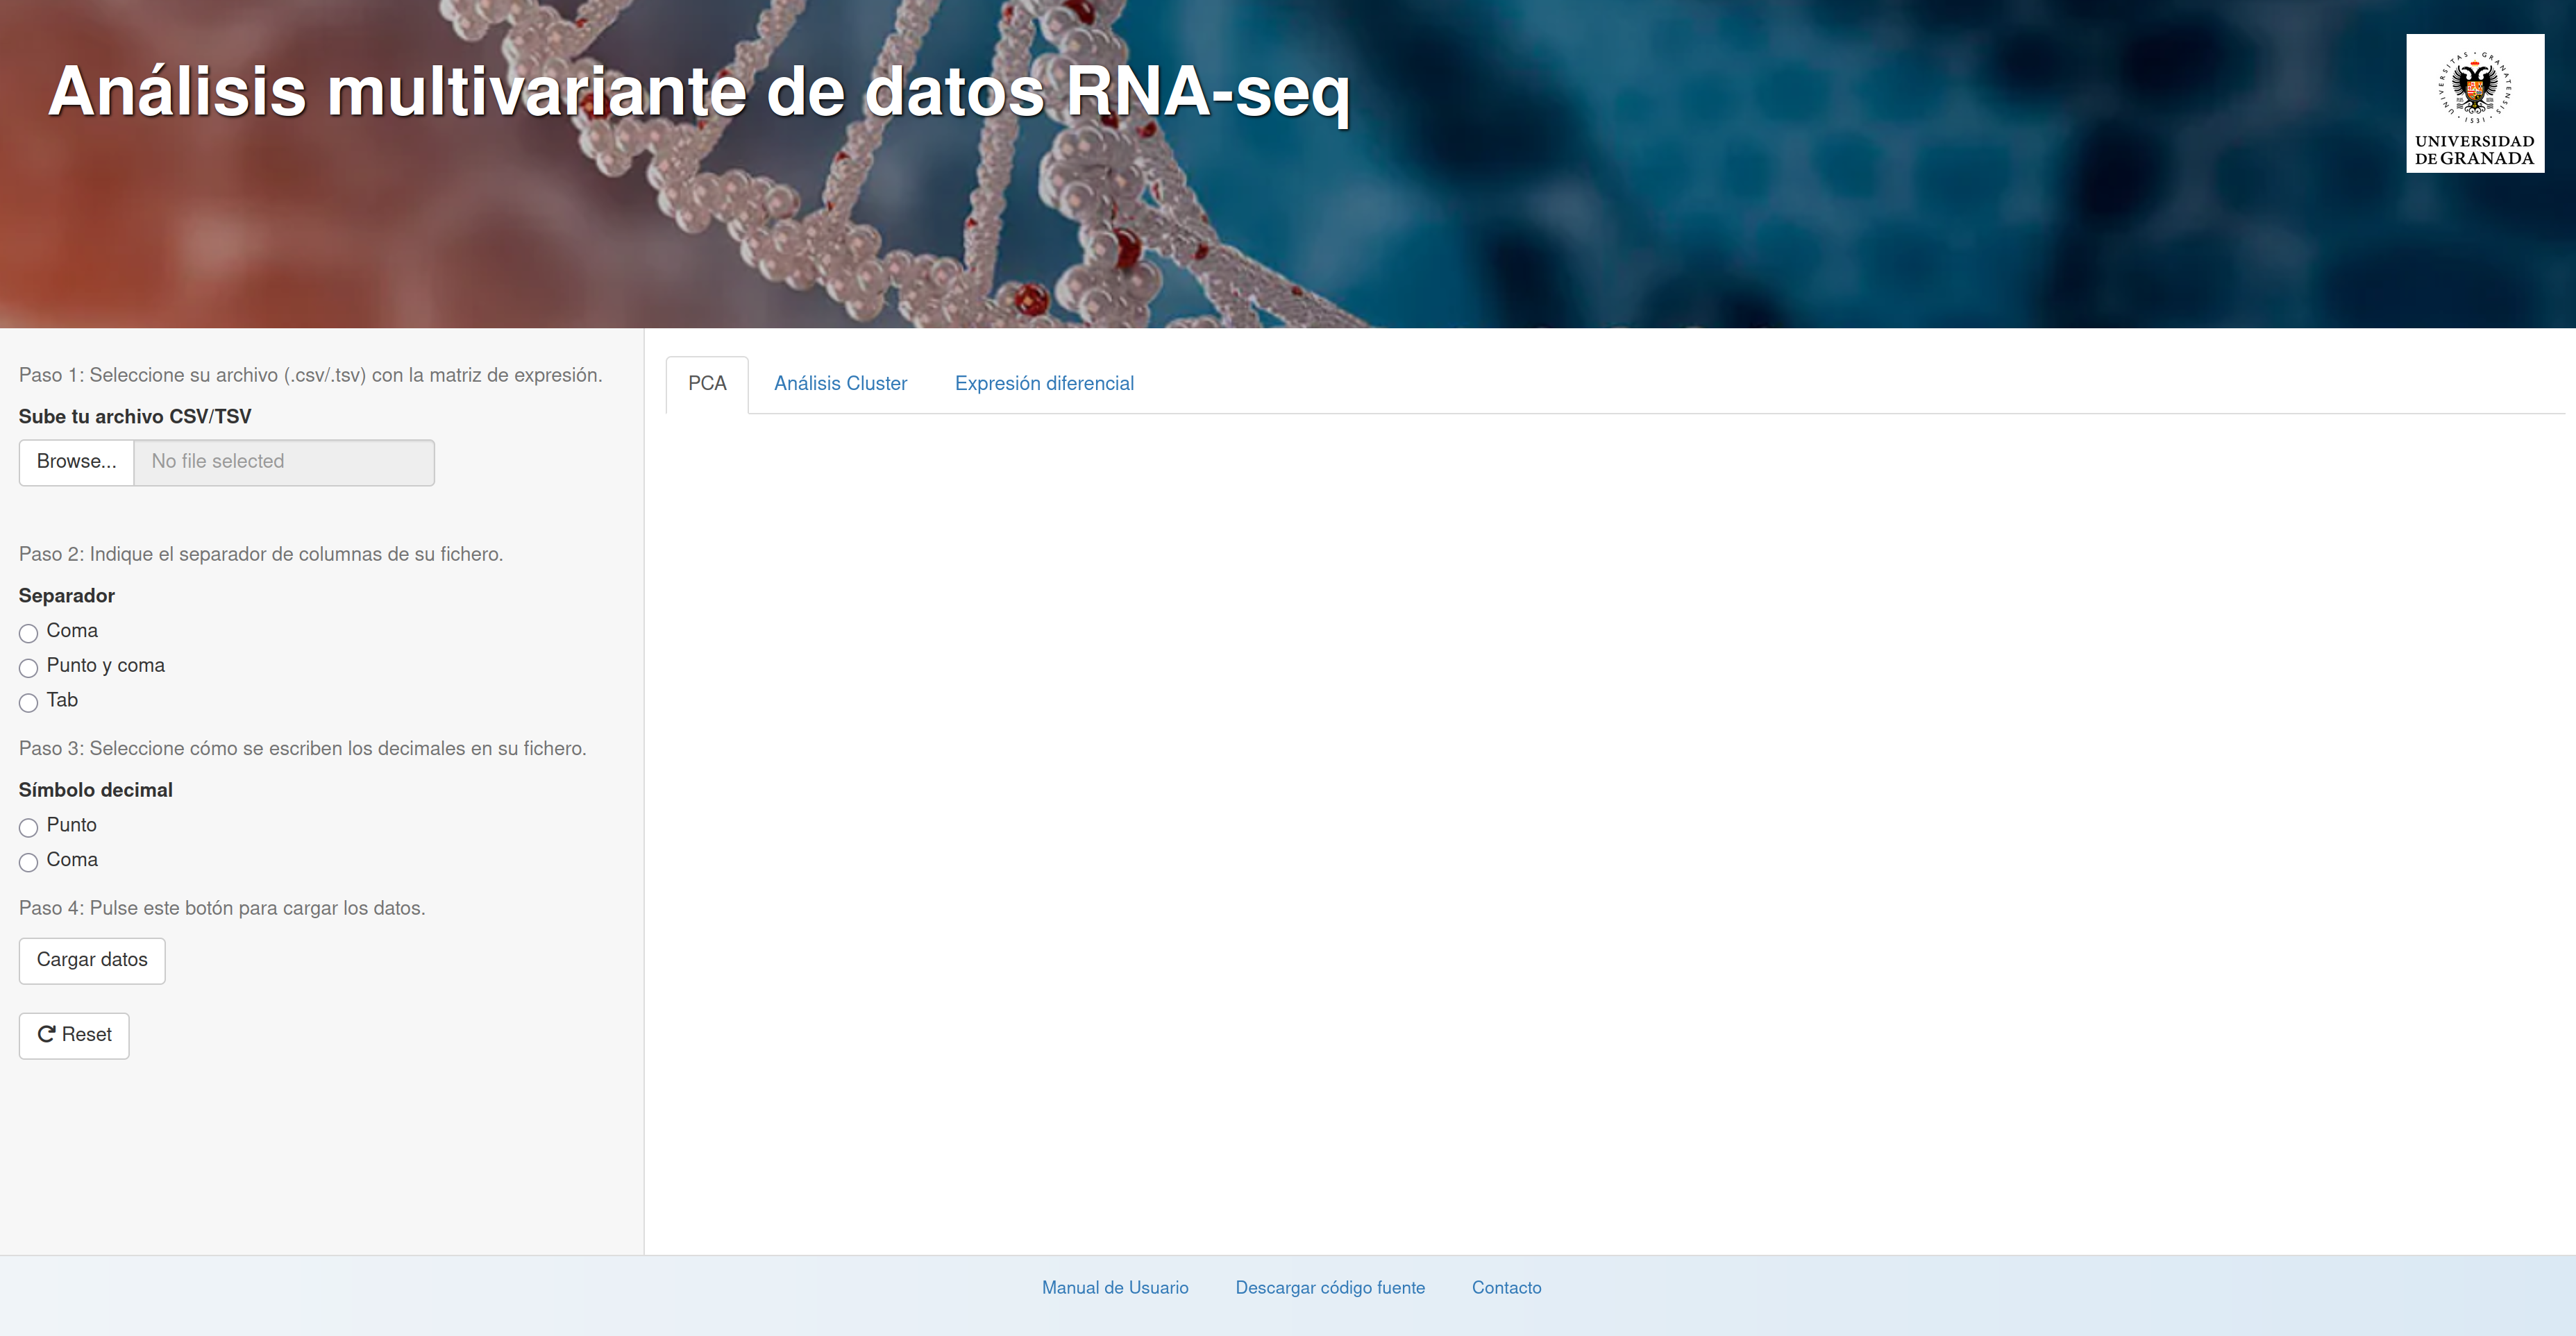
\includegraphics[width=1\textwidth]{../img/app-general.png}
    \caption{Interfaz de usuario (Fuente: elaboración propia).}
\end{figure}

En ella, verá:

\begin{itemize}
    \item Una cabecera con el título de la aplicación y el logo de la Universidad de Granada.
    \item A la izquierda, por debajo de la cabecera, una barra lateral donde podrá:
    \begin{itemize}
        \item Subir su fichero con los datos.
        \item Seleccionar el tipo de separador (coma, punto y coma, tabulador).
        \item Indicar si los números decimales están escritos con coma o punto.
    \end{itemize}
    \item En la parte principal, a la derecha de la barra lateral, verá:
    \begin{itemize}
        \item Un menú con tres botones: PCA, Análisis Cluster, Expresión Diferencial.
        \item Gráficos y resultados que se actualizan según los botones que pulse.
    \end{itemize}
    \item En la panel lateral, tiene a su disposición un botón \textit{Reset} con el que puede deshacer 
    todas las acciones y volverá todo al estado justamente posterior a la carga de datos.
    \item A pie de página verá tres enlaces:
    \begin{itemize}
        \item Un enlace al manual sobre el manejo de la aplicación, que está usted leyendo en estos momentos.
        \item Un enlace de descarga del código fuente desde un repositorio público de \textit{Google Drive}.
        \item Un enlace a una página en la que se muestra información de contacto del desarrollador de la aplicación,
        por si usted tuviera necesidad de comunicarse con el mismo.
    \end{itemize}
\end{itemize}

\subsection{¿Cómo subir los datos?}

Para subir los datos y poder hacer análisis multivariante con ellos, deberá seguir los siguientes pasos:

\begin{itemize}
    \item Haga click en el botón \textit{Subir archivo} de la barra lateral.
    \item Se abrirá el explorador de archivos de su ordenador, donde deberá buscar el archivo que
    contiene los datos.
    \item Seleccione el separador correcto:
    \begin{itemize}
        \item Coma (,) si los valores están separados por comas en el fichero.
        \item Punto y coma (;) si vienen de Excel.
        \item Tabulador si están separados por espacios grandes.
    \end{itemize}
    \item Seleccione si los decimales estarán escritos con punto (.) o coma (,).
    \item Pulse el botón \textit{Cargar datos} para cargar los datos del fichero.
    \item Una vez cargado correctamente, podrá ir a las secciones de análisis.
\end{itemize}

Estos mismos pasos se indican en la propia barra lateral de la interfaz, para guiarlo en todo el proceso, que puede resultar confuso. \newline

Al pulsar el botón \textit{Cargar datos}, necesario pulsarlo para ver los resultados, pueden surgir algunos errores por diferentes causas que se detallan a continuación:

\begin{itemize}
    \item Si no ha seleccionado ningún fichero de su gestor de archivos, obtendrá el mensaje de error de la figura 6.3.
    \begin{figure}[H]
        \centering
        
\includegraphics[width=0.7\textwidth]{../img/err1.png}
        \caption{Error ningún fichero seleccionado (Fuente: elaboración propia).}
    \end{figure}
    \item Si ha seleccionado mal el separador de los distintos registros de su fichero, obtendrá el aviso de la figura 6.4.
    \begin{figure}[H]
        \centering
        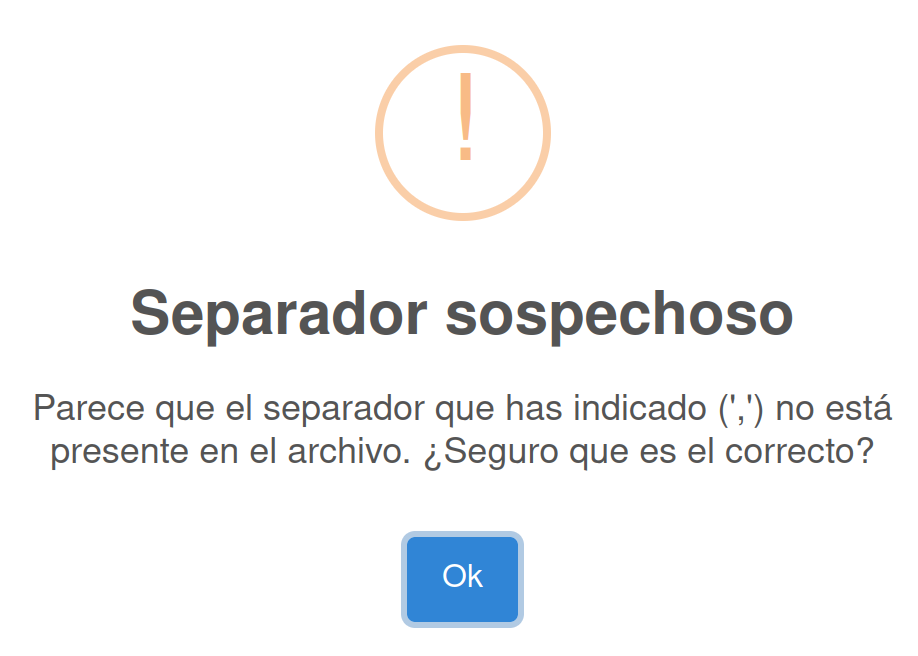
\includegraphics[width=0.7\textwidth]{../img/sep.png}
        \caption{Separador posiblemente erróneo (Fuente: elaboración propia).}
    \end{figure}
    \item Si no ha seleccionado ningún separador, verá el aviso de la figura 6.5.
    \begin{figure}[H]
        \centering
        
\includegraphics[width=0.7\textwidth]{../img/err2.png}
        \caption{Ningún separador seleccionado (Fuente: elaboración propia).}
    \end{figure}
    \item Si no ha seleccionado ningún símbolo decimal, el mensaje que obtendrá será el de la figura 6.6.
    \begin{figure}[H]
        \centering
        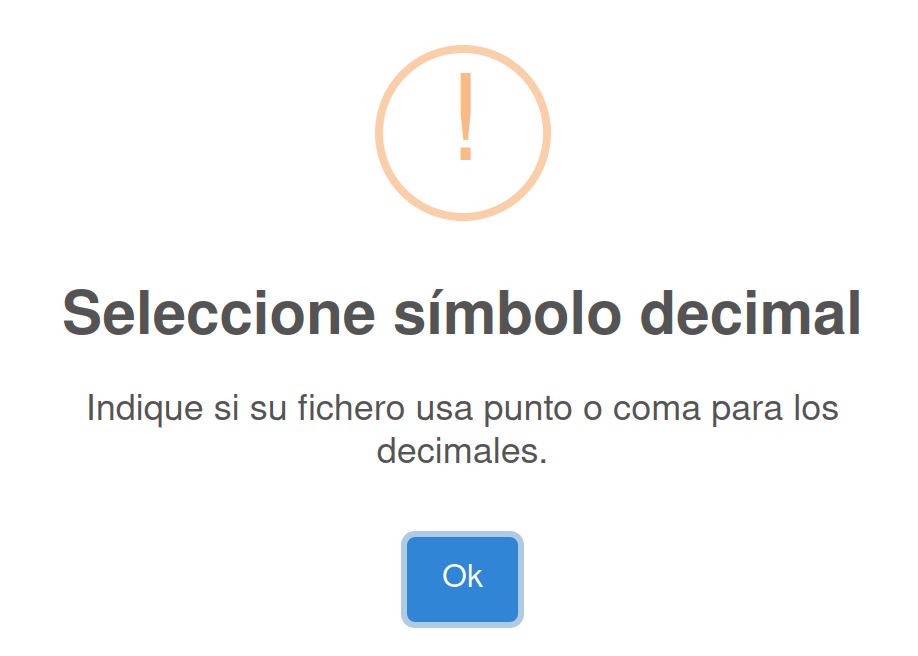
\includegraphics[width=0.7\textwidth]{../img/err3.png}
        \caption{Ningún símbolo decimal seleccionado (Fuente: elaboración propia).}
    \end{figure}
\end{itemize}

\subsection{PCA (Análisis de Componentes Principales)}

Si pulsa sobre el botón \textit{PCA} del menú en línea de la parte principal, se hará todo el proceso correspondiente
al Análisis de Componentes Principales con los datos que haya subido. El PCA sirve para reducir la complejidad de los datos
y poder deshacernos de variables que no aportan mucho al estudio, o lo que es lo mismo, que explican muy poca varianza. Además, 
nos dará pistas acerca de una posible agrupación de los mismos.

\subsubsection{¿Qué verá?}

Tras unos segundos de espera mientras se hacen todos los cálculos, podrá ver un gráfico con puntos de colores que representan las muestras
de su conjunto de datos. Cada eje (PC1,PC2) representa una "combinación" de genes. Verá también otro gráfico que mostrará cuándta información
contiene cada eje (varianza explicada por las distintas componentes principales).

\begin{figure}[H]
    \centering
    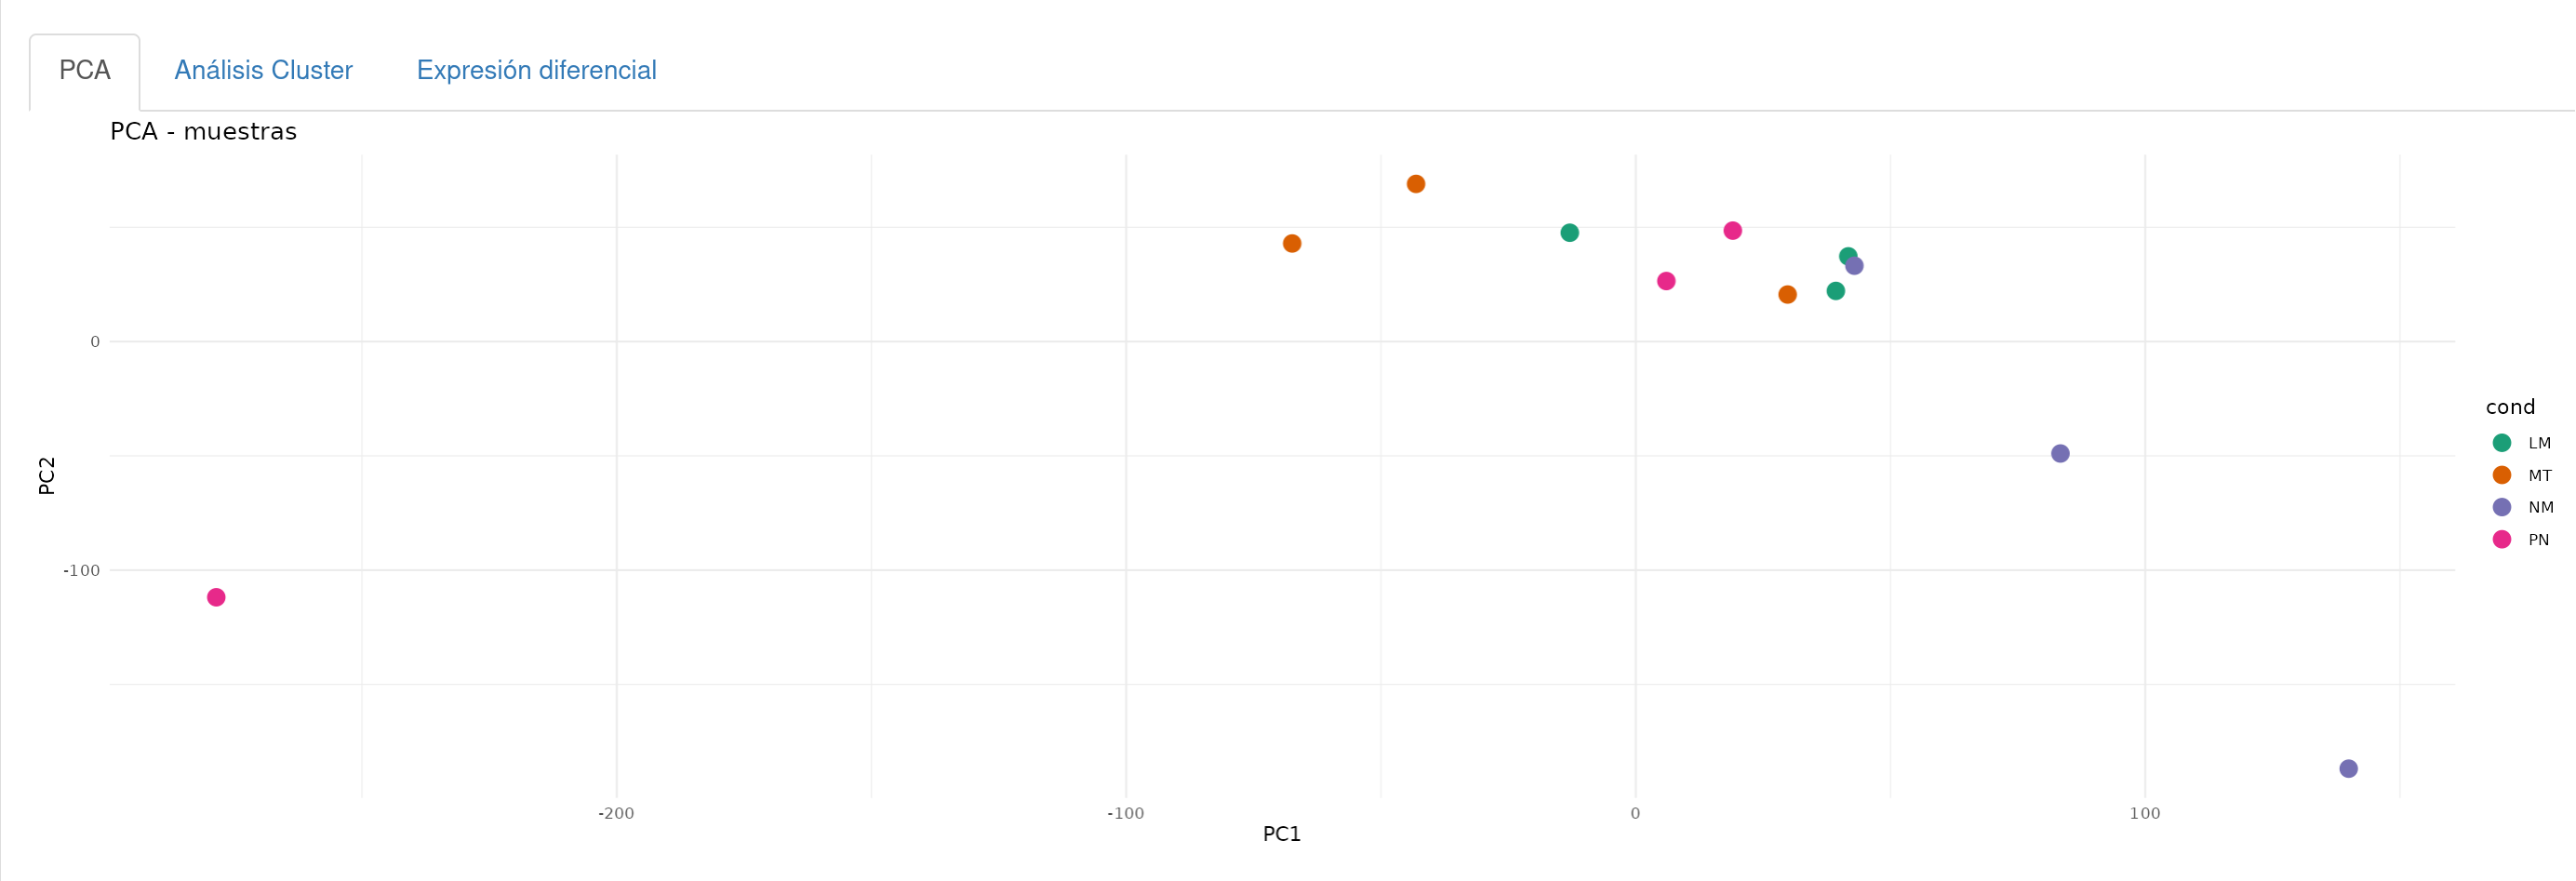
\includegraphics[width=1\textwidth]{../img/pca.png}
    \caption{Análisis de Componentes Principales (PCA) (Fuente: elaboración propia).}
\end{figure}

\subsubsection{¿Qué tiene que hacer usted?}

Nada, solamente tiene que limitarse a cargar los datos. El análisis lo hace automáticamente por debajo. Tras él, con el apoyo
de los gráficos, podrá sacar sus propias conclusiones en función de sus intereses. \newline

Una interpretación básica puede ser la siguiente: 

\begin{itemize}
    \item Si ve puntos juntos: esas muestras se parecen.
    \item Si ve puntos alejados: son diferentes.
    \item Si en el gráfico de la varianza observa que hay barras muy altas en comparación con otras, significa que estas explican
    mucha más información que otras y por tanto, podríamos deshacernos de ellas de cara al análisis.
\end{itemize}

\subsection{Análisis Cluster}

Si pulsa sobre el botón \textit{Análisis Cluster}, es porque quiere realizar clustering sobre los datos cargados. El análisis cluster sirve para 
agrupar las muestras en grupos disjuntos que se llaman \textit{clusters}. Al hacer click, se abren dos opciones:

\begin{itemize}
    \item \textit{Jerárquico:} se muestra un dendrograma (un árbol cuyas hojas son las muestras y que represeta la agrupación jerárquica de las muestras del conjunto de datos, según 
    similitud. Cada bifurcación une dos grupos o elementos similares, y la altura de la unión indica cómo de diferentes son. Se puede cortar a una
    determinada altura para definir el número de clusters).
    \begin{figure}[h]
        \centering
        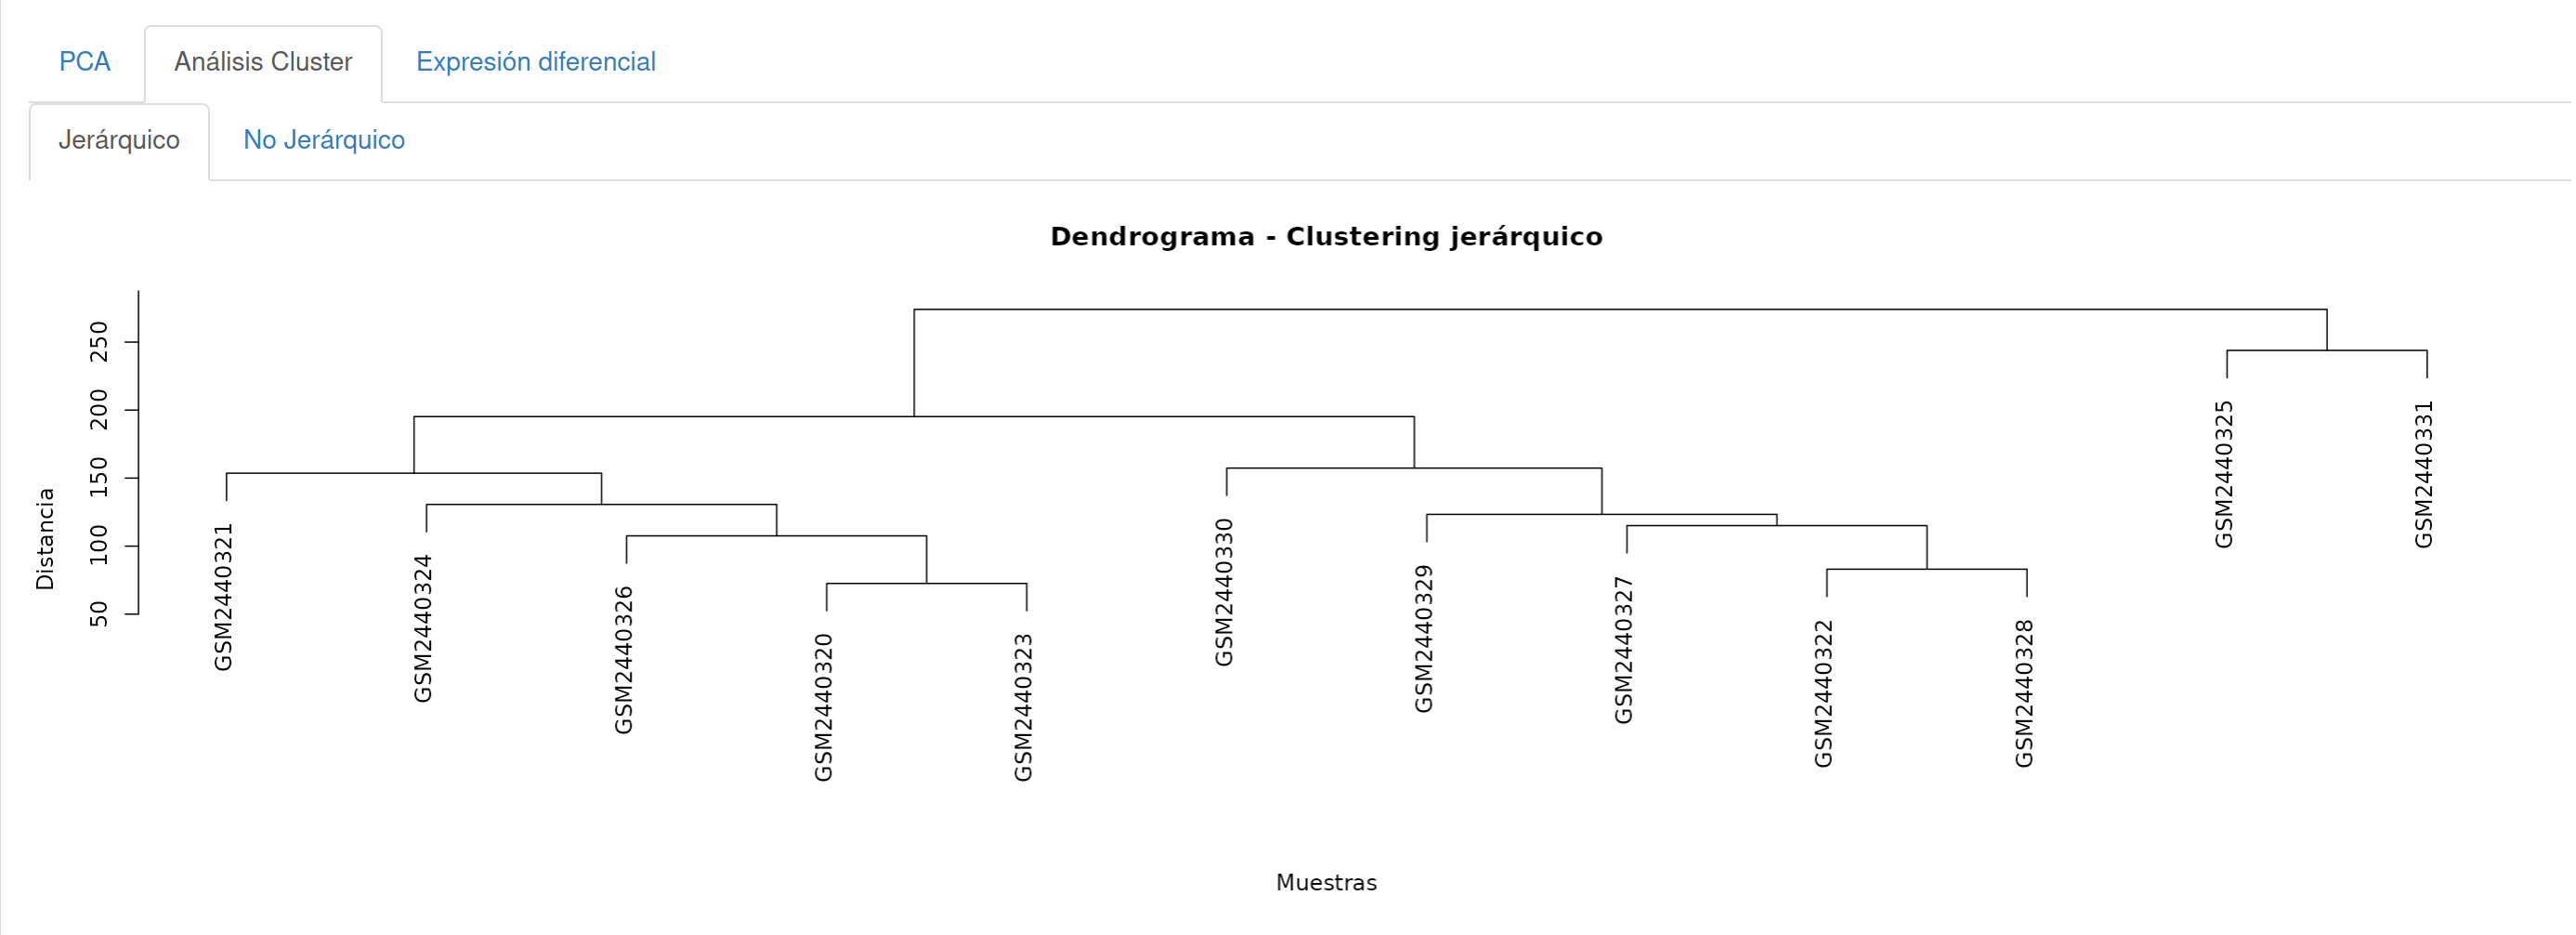
\includegraphics[width=1\textwidth]{../img/jerarquico.png}
        \caption{Análisis cluster jerárquico - Dendrograma (Fuente: elaboración propia).}
    \end{figure}
    \item \textit{No jerárquico:}
    \begin{itemize}
        \item Primero puede determinar cuál podría ser el mejor número de clusters en los que puede agrupar las muestras. Aparecerán dos opciones:
        \begin{itemize}
            \item \textit{Método del codo:} al hacer click, se mostrará un gráfico que tiene una "curva". En el eje X, se disponen distintos valores para 
            el número de clusters (k). En el punto de la gráfica en el que se aprecie un "codo", se encuentra el mejor número de clusters.
            \begin{figure}[H]
                \centering
                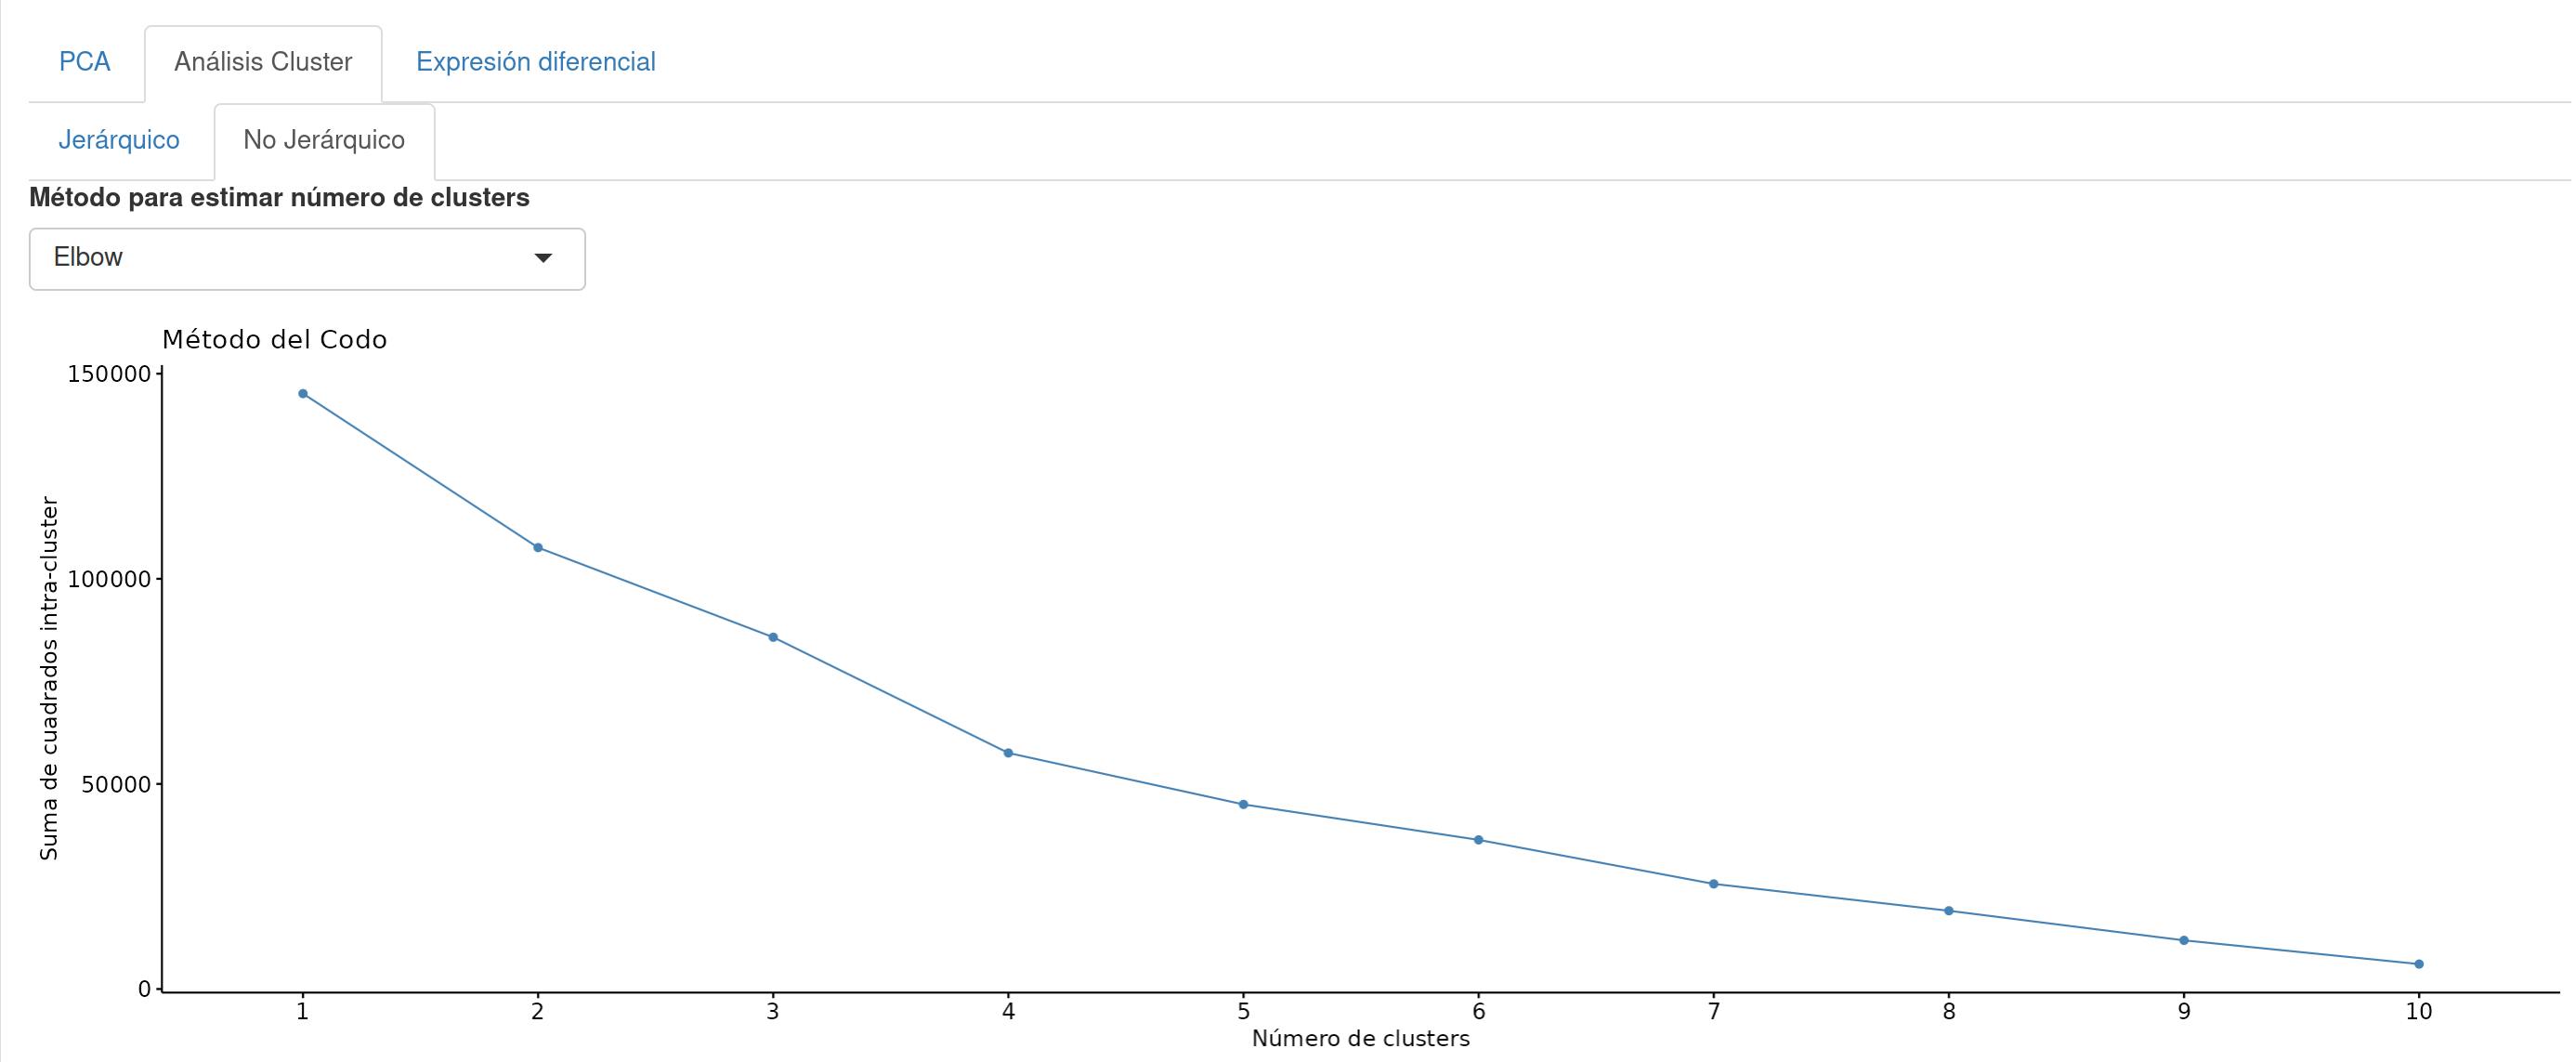
\includegraphics[width=0.8\textwidth]{../img/elbow-app.png}
                \caption{Método del codo (Fuente: elaboración propia).}
            \end{figure}
            \item \textit{Método de la silueta:} muestra también una gráfica de forma que el punto en el que la gráfica alcance su máximo, ese será el candidato
            a número óptimo de clusters.
            \begin{figure}[H]
                \centering
                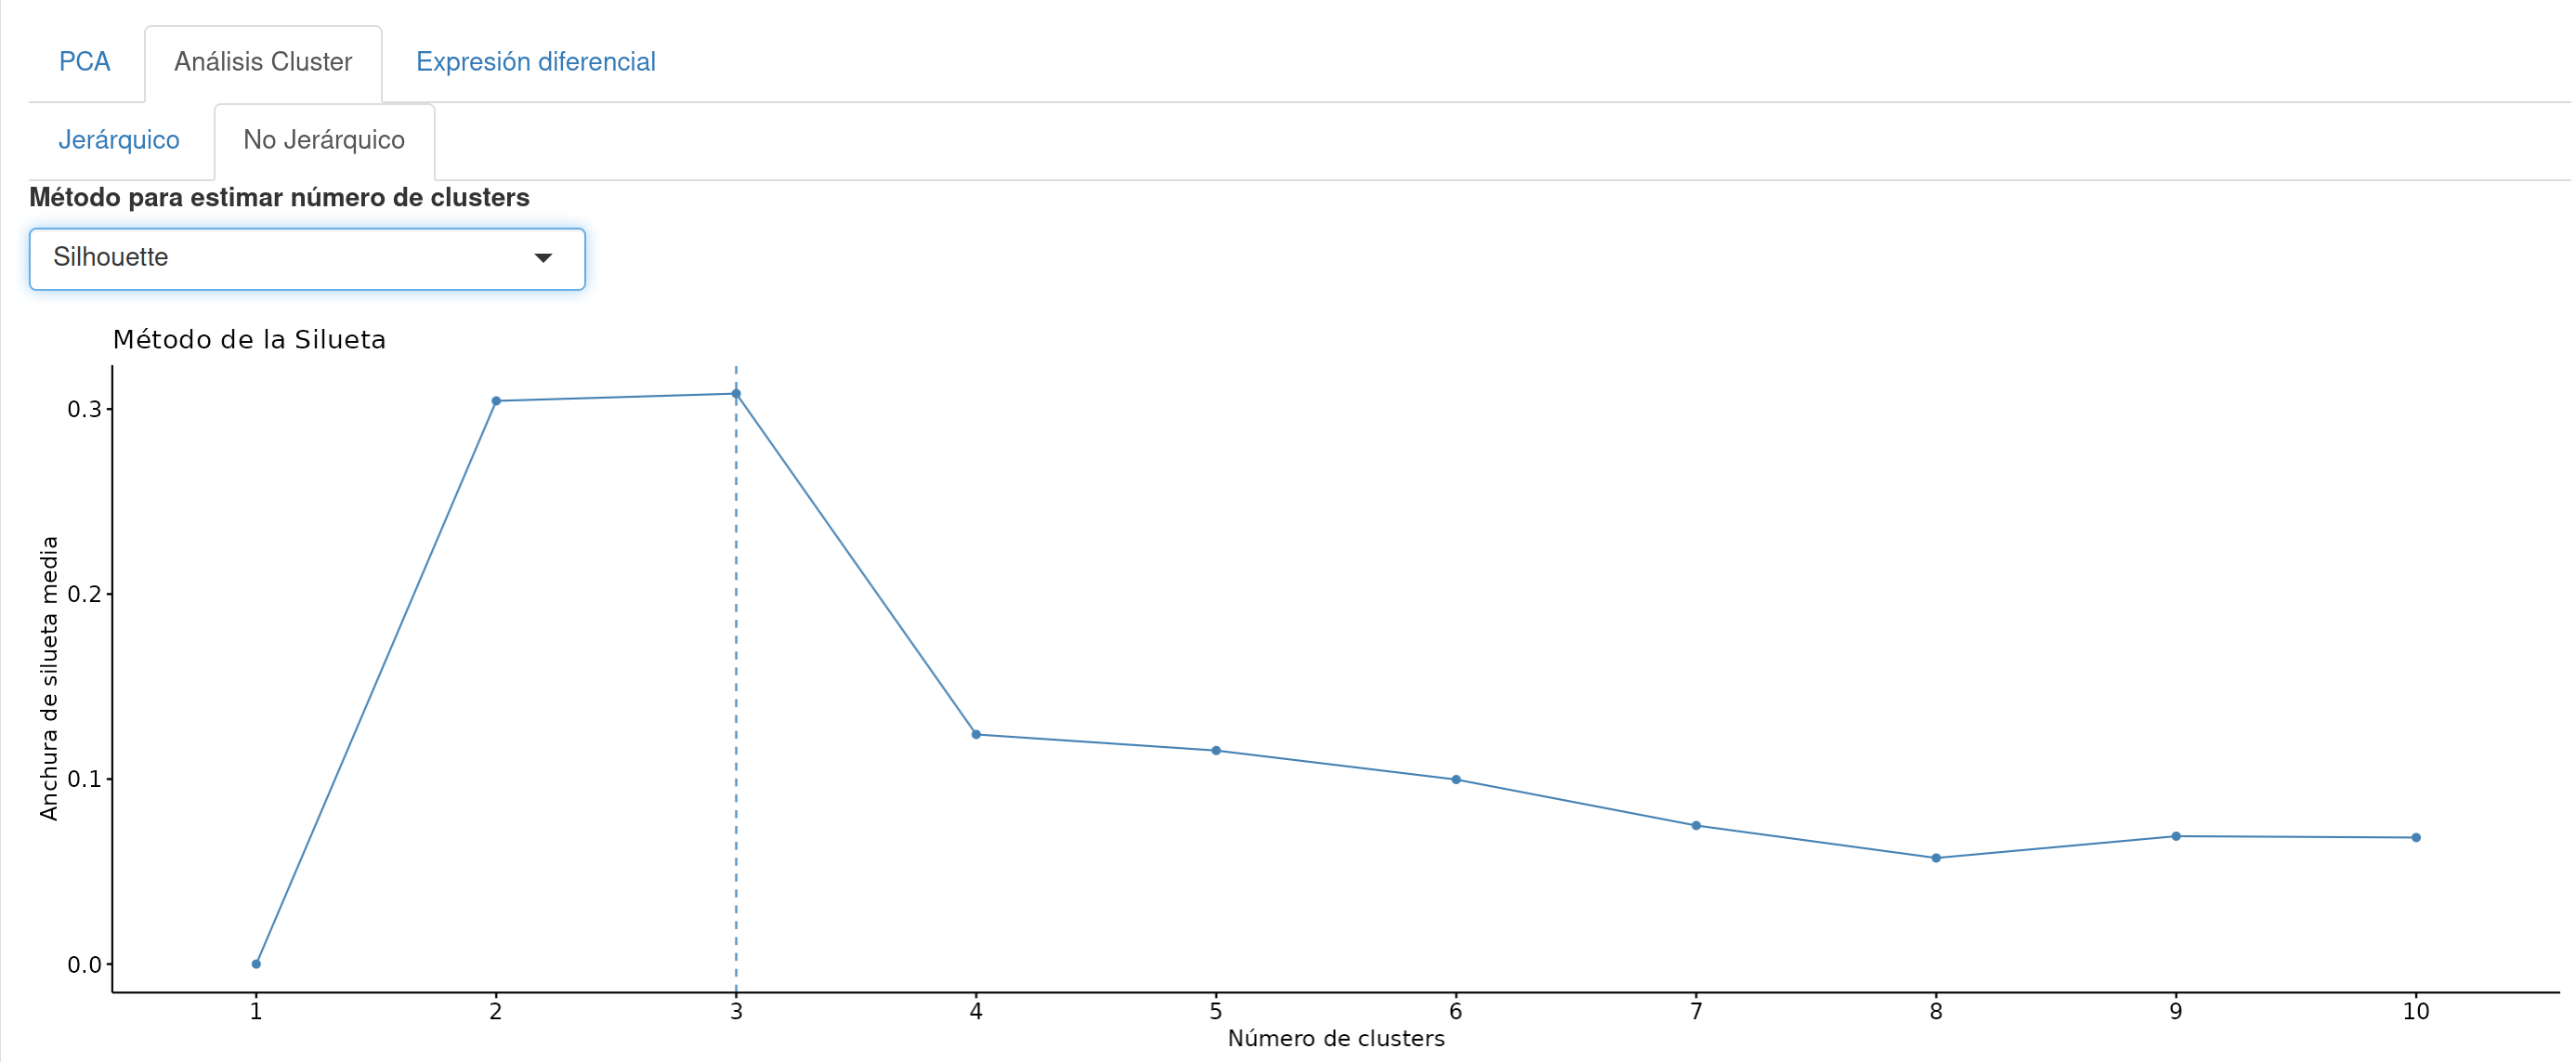
\includegraphics[width=0.8\textwidth]{../img/silueta-app.png}
                \caption{Método de la silueta (Fuente: elaboración propia).}
            \end{figure}
        \end{itemize}
        \item Luego, verá una barra horizontal deslizante con la que podrá elegir el número de clusters con el que aplicar el algoritmo k-means.
        \item Pulsando finalmente sobre el botón \textit{Ejecutar K-means} tras haber escogido el número óptimo de clusters, verá un gráfico con los distintos grupos
        que se habrán formado, en colores diferentes para distinguirlos.
        \begin{figure}[H]
            \centering
            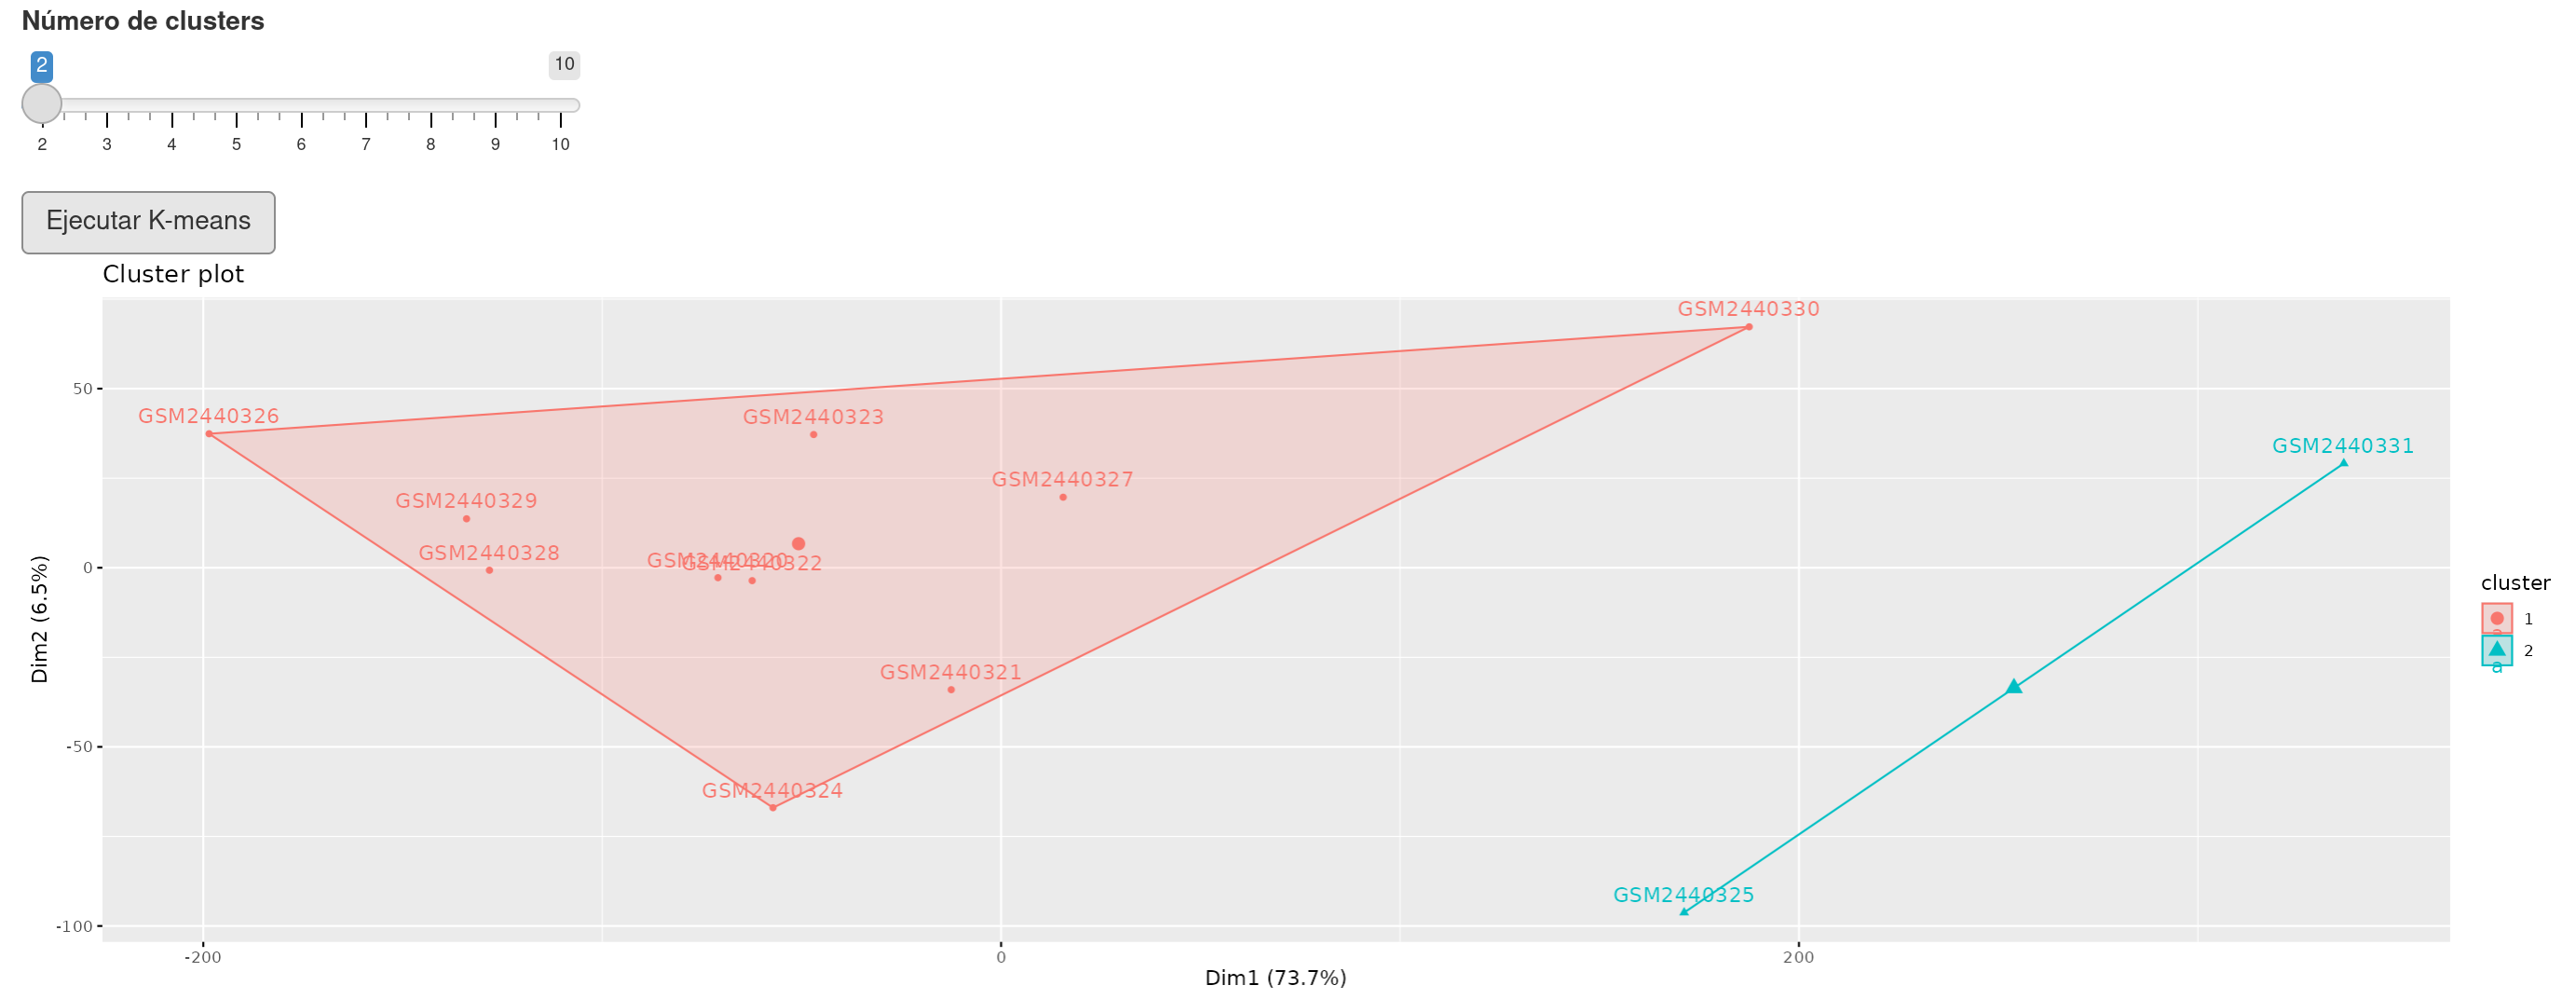
\includegraphics[width=1\textwidth]{../img/kmeans-app.png}
            \caption{Método K-means (Fuente: elaboración propia).}
        \end{figure}
    \end{itemize}
\end{itemize}


\subsection{Análisis de Expresión Diferencial}

Al pulsar el botón \textit{Expresión diferencial}, la aplicación realiza un análisis estadístico para identificar genes cuya expresión varía significativamente entre condiciones.

La tabla resultante muestra las siguientes columnas principales:

\begin{itemize}
  \item \textit{baseMean}: expresión promedio del gen en todas las muestras.
  \item \textit{log2FoldChange}: cambio en la expresión entre condiciones (en escala logarítmica base 2).
  \item \textit{lfcSE}: error estándar del cambio estimado.
  \item \textit{stat}: estadístico del test de comparación.
  \item \textit{pvalue}: probabilidad de que el cambio sea por azar.
  \item \textit{padj}: p-valor ajustado para controlar falsos positivos; valores menores a 0.1 indican significancia.
\end{itemize}

Esta información le permitirá identificar genes con cambios significativos en la expresión entre los grupos analizados.


